% Options for packages loaded elsewhere
% Options for packages loaded elsewhere
\PassOptionsToPackage{unicode}{hyperref}
\PassOptionsToPackage{hyphens}{url}
\PassOptionsToPackage{dvipsnames,svgnames,x11names}{xcolor}
%
\documentclass[
  letterpaper,
  DIV=11,
  numbers=noendperiod]{scrreport}
\usepackage{xcolor}
\usepackage{amsmath,amssymb}
\setcounter{secnumdepth}{5}
\usepackage{iftex}
\ifPDFTeX
  \usepackage[T1]{fontenc}
  \usepackage[utf8]{inputenc}
  \usepackage{textcomp} % provide euro and other symbols
\else % if luatex or xetex
  \usepackage{unicode-math} % this also loads fontspec
  \defaultfontfeatures{Scale=MatchLowercase}
  \defaultfontfeatures[\rmfamily]{Ligatures=TeX,Scale=1}
\fi
\usepackage{lmodern}
\ifPDFTeX\else
  % xetex/luatex font selection
\fi
% Use upquote if available, for straight quotes in verbatim environments
\IfFileExists{upquote.sty}{\usepackage{upquote}}{}
\IfFileExists{microtype.sty}{% use microtype if available
  \usepackage[]{microtype}
  \UseMicrotypeSet[protrusion]{basicmath} % disable protrusion for tt fonts
}{}
\makeatletter
\@ifundefined{KOMAClassName}{% if non-KOMA class
  \IfFileExists{parskip.sty}{%
    \usepackage{parskip}
  }{% else
    \setlength{\parindent}{0pt}
    \setlength{\parskip}{6pt plus 2pt minus 1pt}}
}{% if KOMA class
  \KOMAoptions{parskip=half}}
\makeatother
% Make \paragraph and \subparagraph free-standing
\makeatletter
\ifx\paragraph\undefined\else
  \let\oldparagraph\paragraph
  \renewcommand{\paragraph}{
    \@ifstar
      \xxxParagraphStar
      \xxxParagraphNoStar
  }
  \newcommand{\xxxParagraphStar}[1]{\oldparagraph*{#1}\mbox{}}
  \newcommand{\xxxParagraphNoStar}[1]{\oldparagraph{#1}\mbox{}}
\fi
\ifx\subparagraph\undefined\else
  \let\oldsubparagraph\subparagraph
  \renewcommand{\subparagraph}{
    \@ifstar
      \xxxSubParagraphStar
      \xxxSubParagraphNoStar
  }
  \newcommand{\xxxSubParagraphStar}[1]{\oldsubparagraph*{#1}\mbox{}}
  \newcommand{\xxxSubParagraphNoStar}[1]{\oldsubparagraph{#1}\mbox{}}
\fi
\makeatother


\usepackage{longtable,booktabs,array}
\newcounter{none} % for unnumbered tables
\usepackage{calc} % for calculating minipage widths
% Correct order of tables after \paragraph or \subparagraph
\usepackage{etoolbox}
\makeatletter
\patchcmd\longtable{\par}{\if@noskipsec\mbox{}\fi\par}{}{}
\makeatother
% Allow footnotes in longtable head/foot
\IfFileExists{footnotehyper.sty}{\usepackage{footnotehyper}}{\usepackage{footnote}}
\makesavenoteenv{longtable}
\usepackage{graphicx}
\makeatletter
\newsavebox\pandoc@box
\newcommand*\pandocbounded[1]{% scales image to fit in text height/width
  \sbox\pandoc@box{#1}%
  \Gscale@div\@tempa{\textheight}{\dimexpr\ht\pandoc@box+\dp\pandoc@box\relax}%
  \Gscale@div\@tempb{\linewidth}{\wd\pandoc@box}%
  \ifdim\@tempb\p@<\@tempa\p@\let\@tempa\@tempb\fi% select the smaller of both
  \ifdim\@tempa\p@<\p@\scalebox{\@tempa}{\usebox\pandoc@box}%
  \else\usebox{\pandoc@box}%
  \fi%
}
% Set default figure placement to htbp
\def\fps@figure{htbp}
\makeatother





\setlength{\emergencystretch}{3em} % prevent overfull lines

\providecommand{\tightlist}{%
  \setlength{\itemsep}{0pt}\setlength{\parskip}{0pt}}



 


\KOMAoption{captions}{tableheading}
\makeatletter
\@ifpackageloaded{tcolorbox}{}{\usepackage[skins,breakable]{tcolorbox}}
\@ifpackageloaded{fontawesome5}{}{\usepackage{fontawesome5}}
\definecolor{quarto-callout-color}{HTML}{909090}
\definecolor{quarto-callout-note-color}{HTML}{0758E5}
\definecolor{quarto-callout-important-color}{HTML}{CC1914}
\definecolor{quarto-callout-warning-color}{HTML}{EB9113}
\definecolor{quarto-callout-tip-color}{HTML}{00A047}
\definecolor{quarto-callout-caution-color}{HTML}{FC5300}
\definecolor{quarto-callout-color-frame}{HTML}{acacac}
\definecolor{quarto-callout-note-color-frame}{HTML}{4582ec}
\definecolor{quarto-callout-important-color-frame}{HTML}{d9534f}
\definecolor{quarto-callout-warning-color-frame}{HTML}{f0ad4e}
\definecolor{quarto-callout-tip-color-frame}{HTML}{02b875}
\definecolor{quarto-callout-caution-color-frame}{HTML}{fd7e14}
\makeatother
\makeatletter
\@ifpackageloaded{bookmark}{}{\usepackage{bookmark}}
\makeatother
\makeatletter
\@ifpackageloaded{caption}{}{\usepackage{caption}}
\AtBeginDocument{%
\ifdefined\contentsname
  \renewcommand*\contentsname{Table of contents}
\else
  \newcommand\contentsname{Table of contents}
\fi
\ifdefined\listfigurename
  \renewcommand*\listfigurename{List of Figures}
\else
  \newcommand\listfigurename{List of Figures}
\fi
\ifdefined\listtablename
  \renewcommand*\listtablename{List of Tables}
\else
  \newcommand\listtablename{List of Tables}
\fi
\ifdefined\figurename
  \renewcommand*\figurename{Figure}
\else
  \newcommand\figurename{Figure}
\fi
\ifdefined\tablename
  \renewcommand*\tablename{Table}
\else
  \newcommand\tablename{Table}
\fi
}
\@ifpackageloaded{float}{}{\usepackage{float}}
\floatstyle{ruled}
\@ifundefined{c@chapter}{\newfloat{codelisting}{h}{lop}}{\newfloat{codelisting}{h}{lop}[chapter]}
\floatname{codelisting}{Listing}
\newcommand*\listoflistings{\listof{codelisting}{List of Listings}}
\makeatother
\makeatletter
\makeatother
\makeatletter
\@ifpackageloaded{caption}{}{\usepackage{caption}}
\@ifpackageloaded{subcaption}{}{\usepackage{subcaption}}
\makeatother
\usepackage{bookmark}
\IfFileExists{xurl.sty}{\usepackage{xurl}}{} % add URL line breaks if available
\urlstyle{same}
\hypersetup{
  pdftitle={Metodologia da Transitividade Aplicada nas Escolas do Ensino Médio (E-book)},
  pdfauthor={João Batista Figueiredo Veiga},
  colorlinks=true,
  linkcolor={blue},
  filecolor={Maroon},
  citecolor={Blue},
  urlcolor={Blue},
  pdfcreator={LaTeX via pandoc}}


\title{\textbf{Metodologia da Transitividade Aplicada nas Escolas do
Ensino Médio (\emph{E-book})}}
\usepackage{etoolbox}
\makeatletter
\providecommand{\subtitle}[1]{% add subtitle to \maketitle
  \apptocmd{\@title}{\par {\large #1 \par}}{}{}
}
\makeatother
\subtitle{\textbf{{[}Guia Prático Para Produção de Vídeos
Documentais{]}}}
\author{João Batista Figueiredo Veiga}
\date{2025-08-21}
\begin{document}
\maketitle

\renewcommand*\contentsname{Table of contents}
{
\setcounter{tocdepth}{2}
\tableofcontents
}

\bookmarksetup{startatroot}

\chapter*{APRESENTAÇÃO}\label{apresentauxe7uxe3o}
\addcontentsline{toc}{chapter}{APRESENTAÇÃO}

\markboth{APRESENTAÇÃO}{APRESENTAÇÃO}

O presente e-book tem como propósito organizar, em um formato didático e
acessível, as informações teóricas e práticas sobre a aplicação da
Metodologia da Transitividade no contexto do Ensino Médio. Esta obra é
fruto da sistematização de práticas pedagógicas que buscam aproximar a
escola da realidade dos estudantes, promovendo uma educação pautada no
diálogo, na reflexão crítica e na práxis.

A proposta aqui delineada adapta os passos identificados em
documentos-base sobre a referida metodologia, transpondo-os para uma
prática pedagógica contemporânea: a produção de pequenos vÍdeos
documentais que possam ser utilizados de forma educativa nas redes
sociais (como Reels, TikTok e Shorts). O objetivo não é o domínio
técnico de produção audiovisual ou mero entretenimento, mas visa
utilizar o celular como um instrumento de investigação social e de
leitura crítica do mundo.

\bookmarksetup{startatroot}

\chapter{Introdução}\label{introduuxe7uxe3o}

No contexto do Novo Ensino Médio as atividades educativas que tem a
proposta pedagógica de mediar o conhecimento sistematizado com o
conhecimento sobre a vida prática, permitem que os professores em
diálogo com os alunos tenham uma compreensão mais elaborada sobre a
produção do conhecimento. A proposta de produção do audiovisual adotada,
possui como estratégia o aprofundamento dos saberes dos alunos pela
apropriação dos instrumentos teóricos a partir das vivências sociais, a
fim de criar mecanismos de ação sobre a reflexão feita sobre os
problemas observados no cotidiano, ou seja, através do uso de celular
pelos alunos busca-se uma forma de mediar o conhecimento pelo contexto
vivenciado pelo aluno.

\begin{center}
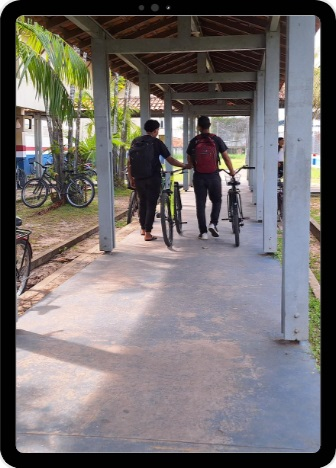
\includegraphics[width=1.94792in,height=\textheight,keepaspectratio]{fig8.jpg}
\end{center}

Esta proposta da Metodologia da Transitividade, orientada pela produção
de minidocumentários e de outras mídias audiovisuais, permite o seu
compartilhamento como conteúdos educacionais nas redes sociais. Também
visa fundamentar a produção de diversos conteúdos de visualização rápida
para postagem nas redes sociais mais utilizadas pelos alunos no
Instagram Reels, TikTok, Facebook Reels, Youtube shorts e Kwai.

A metodologia utilizada nas oficinas nas atividades para o
desenvolvimento do produto, foi a forma encontrada em desenvolver um
produto de forma preliminar, porém considera-se que os resultados dessas
experiências registradas no Guia Prático da Metodologia da
Transitividade, podem ser aplicadas seguindo o formato de oficinas ou
adequada às aulas de sociologia ou à critério de cada professor,
conforme a sua realidade.

A intenção com essa experiência prática é que possamos apresentar uma
metodologia de ensino para que professores trabalhem com os educandos
uma forma prática para aprendizagem de conteúdos sociológicos. Portanto,
o objetivo não é apresentar um plano de aula, mas um Guia Metodológico
onde o professor possa adaptá-lo às suas necessidades de ensino,
adequado à cada contexto onde exerce a docência no suporte à produção de
audiovisual.

\bookmarksetup{startatroot}

\chapter{O Que é a Metodologia da
Transitividade}\label{o-que-uxe9-a-metodologia-da-transitividade}

A Metodologia da Transitividade é uma proposta pedagógica, de forte
inspiração \textbf{Freiriana}, que visa conduzir o estudante da
percepção imediata e ingênua de sua realidade para uma compreensão
estrutural e crítica. A palavra ``transitividade'' refere-se exatamente
a este movimento de transição cognitiva e social, no qual o indivíduo
deixa de ser um mero espectador das contradições a seu redor e passa a
investigá-las ativamente.

\begin{center}
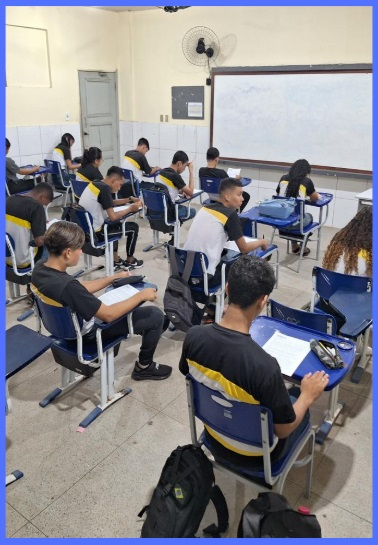
\includegraphics[width=1.84375in,height=\textheight,keepaspectratio]{fig12.jpg}
\end{center}

Seus objetivos educacionais centrais incluem romper com a educação
``bancária'' (aquela que apenas deposita conteúdos no aluno), integrar o
currículo escolar à vida real dos educandos e formar sujeitos capazes de
analisar e intervir em sua realidade.

\section{PrincÍpios Centrais}\label{princuxedpios-centrais}

\begin{itemize}
\tightlist
\item
  \textbf{Diálogo}: Relação horizontal entre educador e educando, onde
  ambos aprendem e investigam juntos.
\item
  \textbf{Leitura Crítica da Realidade}: Partir do contexto vivido pelo
  aluno para desvelar as estruturas sociais.
\item
  \textbf{Articulação Teoria-Prática}: O conhecimento escolar é
  mobilizado para explicar e transformar problemas reais.
\item
  \textbf{Passagem da Ingenuidade à Criticidade}: Superação de opiniões
  baseadas no senso comum por meio da investigação metódica.
\item
  \textbf{Protagonismo Estudantil}: O estudante como autor de seu
  processo de aprendizagem e de leitura social.
\end{itemize}

\begin{tcolorbox}[enhanced jigsaw, arc=.35mm, bottomrule=.15mm, bottomtitle=1mm, breakable, colback=white, colbacktitle=quarto-callout-tip-color!10!white, colframe=quarto-callout-tip-color-frame, coltitle=black, left=2mm, leftrule=.75mm, opacityback=0, opacitybacktitle=0.6, rightrule=.15mm, title=\textcolor{quarto-callout-tip-color}{\faLightbulb}\hspace{0.5em}{Tip}, titlerule=0mm, toprule=.15mm, toptitle=1mm]

``\textbf{EM SÍNTESE} : A Metodologia da Transitividade é um caminho
educacional que usa a investigação do cotidiano para ajudar o aluno a
enxergar as raÍzes dos problemas sociais, transformando a observação
passiva em questionamento crÍtico com autonomia.''.

\end{tcolorbox}

\bookmarksetup{startatroot}

\chapter{Porque Trabalhar Com Vídeos No Ensino
Médio}\label{porque-trabalhar-com-vuxeddeos-no-ensino-muxe9dio}

O uso de dispositivos móveis, especialmente o celular, é uma realidade
inegável na cultura juvenil contemporânea. No entanto, o ambiente
escolar frequentemente enxerga essa tecnologia apenas como uma distração
ou, no máximo, como um recurso passivo para consumo de informações.
Integrar as linguagens audiovisuais próprias das redes sociais ao fazer
pedagógico é uma forma de disputar os sentidos e os usos dessas
tecnologias.

\begin{center}
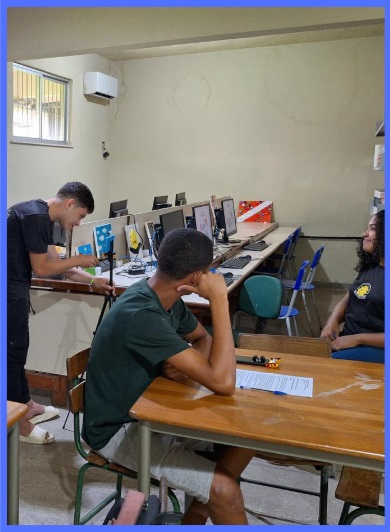
\includegraphics[width=1.88542in,height=\textheight,keepaspectratio]{fig13.jpg}
\end{center}

A proposta aqui apresentada não visa transformar a sala de aula em uma
agência de criação de conteúdo. Pelo contrário, trata-se de utilizar a
câmera do celular como uma ``lente investigativa''. Ao propor que os
estudantes produzam vídeos para as redes sociais, o professor exige
deles processos complexos: observação atenta do espaço, seleção do que é
relevante, elaboração de um roteiro argumentativo e expressão estética
de uma ideia.

Ao registrar o cotidiano, o aluno é forçado a olhar para o que antes lhe
parecia natural. A edição do vídeo se torna um exercício de análise
social, onde a imagem codifica a realidade e a discussão em sala de aula
descodifica suas contradições.

\begin{tcolorbox}[enhanced jigsaw, arc=.35mm, bottomrule=.15mm, bottomtitle=1mm, breakable, colback=white, colbacktitle=quarto-callout-tip-color!10!white, colframe=quarto-callout-tip-color-frame, coltitle=black, left=2mm, leftrule=.75mm, opacityback=0, opacitybacktitle=0.6, rightrule=.15mm, title=\textcolor{quarto-callout-tip-color}{\faLightbulb}\hspace{0.5em}{Tip}, titlerule=0mm, toprule=.15mm, toptitle=1mm]

``\textbf{NA PRÁTICA} : a produção de vídeos para redes sociais na
escola não busca o entretenimento ou a viralização, mas sim o uso da
linguagem audiovisual como ferramenta para investigar, problematizar a
realidade concreta e construir autoria crítica entre os jovens.''

\end{tcolorbox}

\bookmarksetup{startatroot}

\chapter{Passo a Passo
Metodológico}\label{passo-a-passo-metodoluxf3gico}

A aplicação da Metodologia da Transitividade ocorre de forma processual,
estruturada em etapas lógicas que guiam os estudantes da observação à
síntese crítica. Abaixo, detalhamos os nove passos essenciais para a
condução do trabalho.

{\def\LTcaptype{none} % do not increment counter
\begin{longtable}[]{@{}
  >{\raggedright\arraybackslash}p{(\linewidth - 2\tabcolsep) * \real{0.4752}}
  >{\raggedright\arraybackslash}p{(\linewidth - 2\tabcolsep) * \real{0.5248}}@{}}
\toprule\noalign{}
\endhead
\bottomrule\noalign{}
\endlastfoot
\begin{minipage}[t]{\linewidth}\raggedright
\begin{enumerate}
\def\labelenumi{\arabic{enumi}.}
\item
  \textbf{Organização Inicial};
\item
  \textbf{Diálogo com Alunos};
\item
  \textbf{Diálogo com a Realidade};
\item
  \textbf{A Investigação da Àrea de Estudo};
\item
  \textbf{Codificação das Experiências Sociais};
\item
  \textbf{Diálogos DesCodificados};
\item
  \textbf{Redução Temática};
\item
  \textbf{Desenvolvimento em Sala de Aula};
\item
  \textbf{Apresentação dos Vídeos e Avaliação};
\end{enumerate}
\end{minipage} &

\includegraphics[width=2.82292in,height=\textheight,keepaspectratio]{images/clipboard-1725403957.jpeg} \\
\end{longtable}
}

\bookmarksetup{startatroot}

\chapter{Detlhamento das Etapas}\label{detlhamento-das-etapas}

\section{Organização Inicial}\label{organizauxe7uxe3o-inicial}

\textbf{Objetivo}: O professor apresenta a proposta, explica que a
atividade não é apenas ``gravar um vídeo'', mas investigar a realidade e
transformá-la em leitura crítica. Também organiza grupos, define prazos,
conversa sobre uso responsável de imagem, ética digital e finalidade
pedagógica da produção.

\textbf{O Que os Estudantes Fazem}: Compreendem a intencionalidade do
trabalho formam suas equipes de investigação e começam a debater
possíveis temas.

\begin{center}
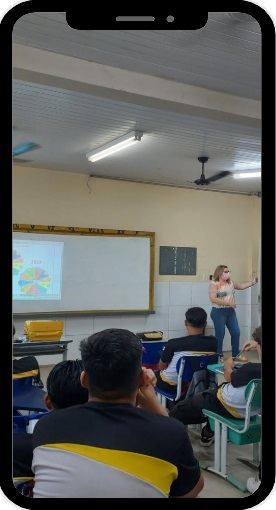
\includegraphics[width=1.40625in,height=\textheight,keepaspectratio]{fig4.jpg}
\end{center}

\section{Diálogos com os Alunos}\label{diuxe1logos-com-os-alunos}

Nesse momento inicial, o professor promove uma roda de conversa para
ouvir os estudantes sobre questões que merecem ser discutidas. Inicia
com perguntas, em vez de começar pelo conteúdo pronto, começa pela
experiência vivida pelos alunos.

Esse movimento aparece no documento como um momento de aproximação e
escuta, em coerência com o processo educativo dialógico.

\begin{center}
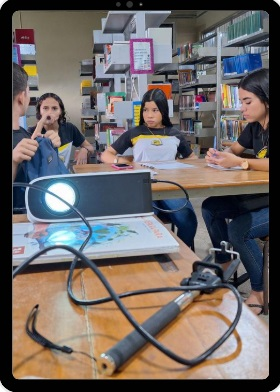
\includegraphics[width=1.90625in,height=\textheight,keepaspectratio]{fig9.jpg}
\end{center}

\subsection{Exemplos de Perguntas
Problematizadoras:}\label{exemplos-de-perguntas-problematizadoras}

\begin{itemize}
\tightlist
\item
  O que mais incomoda vocês na escola ou no bairro?
\item
  Que situações todo mundo vê, mas quase ninguém discute?
\item
  Se vocês pudessem denunciar, explicar ou conscientizar sobre algo em 1
  minuto, o que seria?
\item
  Que tipo de vídeo vocês consomem nas redes que prende atenção?
\end{itemize}

\subsection{Exemplo de Atividade em
Sala}\label{exemplo-de-atividade-em-sala}

Cada aluno escreve em um post-it ou formulário:

\begin{enumerate}
\def\labelenumi{\arabic{enumi}.}
\tightlist
\item
  um problema que observa;
\item
  uma pergunta que gostaria de investigar;
\item
  uma ideia de vídeo curto sobre esse problema.
\end{enumerate}

\subsection{Produto Esperado}\label{produto-esperado}

\begin{itemize}
\tightlist
\item
  Mapa de interesses da turma.
\end{itemize}

\section{Diálogos com a Realidade}\label{diuxe1logos-com-a-realidade}

Dialogar com os alunos sobre o olhar a realidade de forma mais atenta,
saindo de opiniões genéricas e indo para observações concreta.

\begin{center}
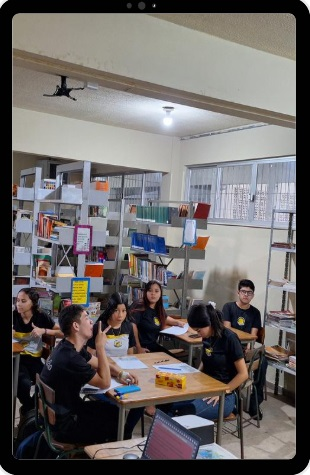
\includegraphics[width=1.78125in,height=\textheight,keepaspectratio]{fig10.jpg}
\end{center}

O professor conduz uma atividade de leitura do espaço escolar ou do
entorno. O importante aqui é deslocar o olhar:

\begin{itemize}
\tightlist
\item
  ``o que vemos?'',
\item
  ``quem aparece?'',
\item
  ``quem não aparece?'',
\item
  ``que contradições existem?''.
\end{itemize}

No documento, esse momento prepara os estudantes para observar
criticamente seu contexto antes do registro audiovisual.

\subsection{Exemplos de Perguntas
Problematizadoras:}\label{exemplos-de-perguntas-problematizadoras-1}

\begin{itemize}
\tightlist
\item
  O que mais incomoda vocês na escola ou no bairro?
\item
  Que situações todo mundo vê, mas quase ninguém discute?
\item
  Se vocês pudessem denunciar, explicar ou conscientizar sobre algo em 1
  minuto, o que seria?
\item
  Que tipo de vídeo vocês consomem nas redes que prende atenção?
\end{itemize}

\subsection{Exemplo de Atividade
Prática:}\label{exemplo-de-atividade-pruxe1tica}

Se o tema for lixo no entorno da escola, os alunos podem observar:

\begin{itemize}
\tightlist
\item
  onde há mais lixo acumulado;
\item
  em que horários isso acontece;
\item
  se há lixeiras suficientes;
\item
  quem é responsabilizado pelo problema;
\item
  como os moradores ou estudantes percebem isso.
\end{itemize}

\subsection{Sugestão de Recurso}\label{sugestuxe3o-de-recurso}

\begin{itemize}
\tightlist
\item
  Use uma ficha simples de observação com três colunas:

  \begin{itemize}
  \tightlist
  \item
    o que vimos?
  \item
    por que isso acontece?
  \item
    que pergunta isso gera?
  \end{itemize}
\end{itemize}

\subsection{Produto Esperado}\label{produto-esperado-1}

\begin{itemize}
\tightlist
\item
  Registro de observações e primeiras hipóteses.
\end{itemize}

\section{Investigação da Área de
Estudo}\label{investigauxe7uxe3o-da-uxe1rea-de-estudo}

É o momento de construir o levantamento preliminar do tema escolhido de
modo mais sistemático.

O professor dialoga com os alunos sobre a coleta inicial de relatos,
cenas, imagens e falas significativas. É a 1ª etapa da investigação
temática, quando ocorre o levantamento preliminar da realidade estudada.

Os estudantes definem o que querem descobrir, quem pretendem entrevistar
e em quais espaços farão as filmagens.

\begin{center}
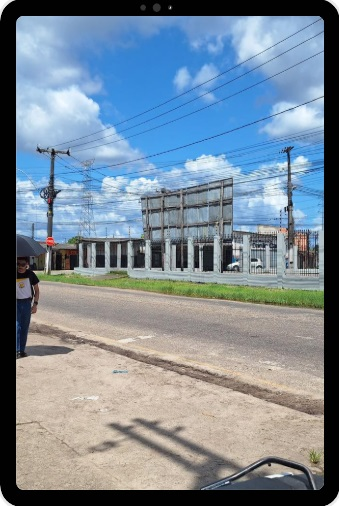
\includegraphics[width=1.8125in,height=\textheight,keepaspectratio]{fig5.jpg}
\end{center}

\subsection{Exemplo de Temática que pode
surgir:}\label{exemplo-de-temuxe1tica-que-pode-surgir}

``As dificuldades de mobilidade que os alunos enfrentam para chegar à
escola''.

\subsection{Miniatividade
Investigativa}\label{miniatividade-investigativa}

\begin{itemize}
\tightlist
\item
  Qual é o problema?
\item
  Onde ele aparece?
\item
  Quem é afetado?
\item
  Como ele costuma ser explicado?
\item
  O que ainda precisamos descobrir?
\end{itemize}

\subsection{Produto Esperado}\label{produto-esperado-2}

\begin{itemize}
\tightlist
\item
  Um dossiê inicial do tema com anotações, fotos, falas e perguntas
\end{itemize}

\section{Codificação das Experiências
Sociais}\label{codificauxe7uxe3o-das-experiuxeancias-sociais}

É o momento de transformar situações reais em materiais de registro:
fotos, áudios, vídeos, entrevistas, cenas do cotidiano.

De acordo com a concepção freiriana, a codificação consiste em registrar
aspectos da realidade para que depois eles possam ser analisados. Essa é
a fase da captação de ``retratos'' da realidade.

\begin{center}
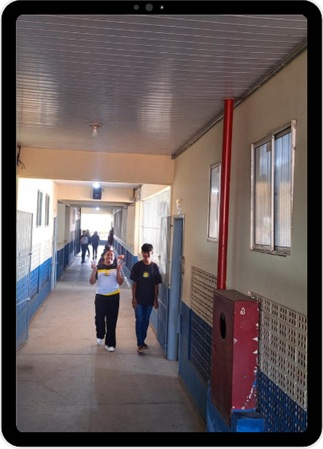
\includegraphics[width=1.78125in,height=\textheight,keepaspectratio]{fig1.jpg}
\end{center}

O professor com os alunos detalham as noções simples tais como:

\begin{itemize}
\tightlist
\item
  Técnicas de Enquadramento;
\item
  Plano Aberto, Médio e Close;
\item
  Captação de áudio;
\item
  Iluminação;
\item
  Gravação na vertical ou na horizontal para Reels/TikTok/Shorts;
\item
  Autorização de imagem quando houver entrevistas gravadas.
\end{itemize}

\subsection{Atividades que as Equipes podem
Realizar}\label{atividades-que-as-equipes-podem-realizar}

\begin{itemize}
\tightlist
\item
  Coletar as opiniões de colegas;
\item
  Registrar a chegada dos alunos;
\item
  Enquete sobre os riscos identificados no trajeto;
\item
  Fazer fotos e vídeos das vias do bairro, das ciclovias, faixas de
  travessia de pedestres, pontos de ônibus, etc;
\item
  Filmar o trânsito no entorno da escola.
\end{itemize}

\subsection{Exemplos de Gravações que podem
Realizar}\label{exemplos-de-gravauxe7uxf5es-que-podem-realizar}

\begin{itemize}
\tightlist
\item
  Gravação de alunos nos pontos de ônibus;
\item
  Gravação de alunos que vem de bicicletas pelas ciclofaixas;
\item
  Entrevistas curtas com estudantes;
\item
  Cenas de deslocamento de alunos pedestres;
\item
  Fla em off com dados ou reflexões.
\end{itemize}

\subsection{Modelo a ser utilizado (vídeo denúncia em 45
seg)}\label{modelo-a-ser-utilizado-vuxeddeo-denuxfancia-em-45-seg}

\begin{enumerate}
\def\labelenumi{\arabic{enumi}.}
\tightlist
\item
  Abertura com pergunta forte;
\item
  Cenas do problema;
\item
  Fala de 2 colegas;
\item
  Dado simples;
\item
  Conclusão com proposta.
\end{enumerate}

\subsection{Produto Esperado:}\label{produto-esperado-3}

\begin{itemize}
\tightlist
\item
  Banco de imagens e vídeos do grupo.
\end{itemize}

\section{Diálogos Descodificadores}\label{diuxe1logos-descodificadores}

É o momento no qual educandos e educadores vão interpretar criticamente
o material.

Esta é uma etapa decisiva. O professor exibe os registros e conduz a
análise coletiva: o que o vídeo mostra? O que ele esconde? Que
contradições aparecem? Que causas estruturais podem estar por trás? No
documento, esta etapa é chamada de diálogos descodificadores e serve
para sair da aparência e chegar à problematização crítica.

\subsection{Perguntas de
Descodificação}\label{perguntas-de-descodificauxe7uxe3o}

\begin{itemize}
\tightlist
\item
  O que aparece com mais força nas imagens?
\item
  Que problema social está sendo revelado?
\item
  Isso é um caso isolado ou algo recorrente?
\item
  Quem ganha e quem perde com essa situação?
\item
  Como a escola, a comunidade ou o poder público entram nisso?
\item
  O vídeo reforça apenas questões comportamentais ou ajuda a pensar como
  um problema coletivo?
\end{itemize}

\subsection{Exemplo que podem ser
Problematizados}\label{exemplo-que-podem-ser-problematizados}

No caso a codificação tenha sido os alunos no trânsito, pois a partir
desse exemplo podem surgir outras temáticas:

\begin{itemize}
\tightlist
\item
  Os problemas enfrentados no trânsito são apenas de imprudência dos
  condutores?
\item
  Quais riscos os alunos identificam no trajeto até a escola?
\item
  As vias do bairro são seguras e bem sinalizadas?
\item
  Quem é responsável pelo trânsito no município?
\end{itemize}

\subsection{Produto Esperado}\label{produto-esperado-4}

\begin{itemize}
\tightlist
\item
  Uma síntese crítica do tema em 5 a 8 frases
\end{itemize}

\begin{tcolorbox}[enhanced jigsaw, arc=.35mm, bottomrule=.15mm, bottomtitle=1mm, breakable, colback=white, colbacktitle=quarto-callout-tip-color!10!white, colframe=quarto-callout-tip-color-frame, coltitle=black, left=2mm, leftrule=.75mm, opacityback=0, opacitybacktitle=0.6, rightrule=.15mm, title=\textcolor{quarto-callout-tip-color}{\faLightbulb}\hspace{0.5em}{Tip}, titlerule=0mm, toprule=.15mm, toptitle=1mm]

``\textbf{OUTRO EXEMPLO PRÁTICO:} Caso o tema fosse a Merenda Escolar.
Após ver os registros codificados, a turma poderia discutir:

\begin{itemize}
\tightlist
\item
  O Problema é quantidade, qualidade ou organização da escola?
\item
  Os Estudantes só reclamam ou conseguem explicar melhor a questão?
\item
  O Vídeo está culpando pessoas específicas ou analisando uma situação
  maior?
\item
  Como Apresentar o problema com responsabilidade?
\end{itemize}

\end{tcolorbox}

\section{Redução Temática}\label{reduuxe7uxe3o-temuxe1tica}

A finalidade é recortar o foco central do vídeo para que ele fique
claro, coerente e pedagógico.

Depois da discussão, o professor ajuda os alunos a definir qual aspecto
do problema será abordado. Nessa etapa de redução temática é o momento
em que o tema investigado é delimitado para ganhar forma educativa.

\subsection{Perguntas de
Descodificação}\label{perguntas-de-descodificauxe7uxe3o-1}

\begin{itemize}
\tightlist
\item
  O que aparece com mais força nas imagens?
\item
  Que problema social está sendo revelado?
\item
  Isso é um caso isolado ou algo recorrente?
\item
  Quem ganha e quem perde com essa situação?
\item
  Como a escola, a comunidade ou o poder público entram nisso?
\item
  O vídeo reforça apenas questões comportamentais ou ajuda a pensar como
  um problema coletivo?
\end{itemize}

\subsection{Exemplo de Temas para
Codificação}\label{exemplo-de-temas-para-codificauxe7uxe3o}

``saúde mental na escola'', Recortes que poderiam ser possíveis nessa
etapa:

\begin{itemize}
\tightlist
\item
  Pressão por Desempenho;
\item
  Excesso de Tarefas;
\item
  Falta de Escuta;
\item
  Impacto das Redes Sociais;
\item
  Comparação entre Colegas.
\end{itemize}

\begin{tcolorbox}[enhanced jigsaw, arc=.35mm, bottomrule=.15mm, bottomtitle=1mm, breakable, colback=white, colbacktitle=quarto-callout-tip-color!10!white, colframe=quarto-callout-tip-color-frame, coltitle=black, left=2mm, leftrule=.75mm, opacityback=0, opacitybacktitle=0.6, rightrule=.15mm, title=\textcolor{quarto-callout-tip-color}{\faLightbulb}\hspace{0.5em}{Tip}, titlerule=0mm, toprule=.15mm, toptitle=1mm]

\textbf{ATIVIDADE PRÁTICA}

\begin{itemize}
\item
  Cada grupo completa esta frase: ``Nosso vídeo vai mostrar
  que\_\_\_\_\_\_\_\_\_, porque observamos \_\_\_\_\_\_\_\_\_\_\_\_\_, e
  queremos que o público reflita sobre\_\_\_\_\_\_\_\_\_\_\_.''
\item
  \textbf{Produto Esperado}

  \begin{itemize}
  \tightlist
  \item
    Tema final com a mensagem central do vídeo.
  \end{itemize}
\end{itemize}

\end{tcolorbox}

\section{Desenvolvimento em Sala de
Aula}\label{desenvolvimento-em-sala-de-aula}

É a etapa de confecção do material didático, com a finalidade de
roteirizar, editar e finalizar o vídeo.

Essa etapa corresponde ao momento em que o material se transforma em
produto didático. Essa etapa do desenvolvimento em sala surge com a
confecção do material audiovisual final.

\subsection{Exemplos de Estrutura/Roteiro para vídeo
curto:}\label{exemplos-de-estruturaroteiro-para-vuxeddeo-curto}

\begin{enumerate}
\def\labelenumi{\arabic{enumi}.}
\tightlist
\item
  \textbf{Modelo 1} --- Vídeo Explicativo
\end{enumerate}

\begin{itemize}
\tightlist
\item
  Gancho inicial: ``Você já percebeu que\ldots?''
\item
  Apresentação do problema.
\item
  Imagens do cotidiano.
\item
  Duas falas ou dados curtos.
\item
  Análise crítica.
\end{itemize}

2.\textbf{Modelo 2} --- Minidocumentário Curto para Rede Social:

\begin{itemize}
\tightlist
\item
  Cena inicial de impacto.
\item
  Narração breve.
\item
  Entrevista curta.
\item
  Contraste entre falas/imagens.
\end{itemize}

\subsection{Exemplo para Confeccionar em
Sala.}\label{exemplo-para-confeccionar-em-sala.}

\begin{itemize}
\tightlist
\item
  Tema: ``Lixo no Bairro''

  \begin{itemize}
  \tightlist
  \item
    Roteiro em 60 segundos:

    \begin{itemize}
    \tightlist
    \item
      0--5s: imagem do problema e pergunta;
    \item
      5--20s: cenas do entorno;
    \item
      20--35s: fala de morador ou estudante;
    \item
      35--50s: interpretação do grupo;
    \item
      50--60s: proposta de reflexão/ação.
    \end{itemize}
  \end{itemize}
\end{itemize}

\begin{tcolorbox}[enhanced jigsaw, arc=.35mm, bottomrule=.15mm, bottomtitle=1mm, breakable, colback=white, colbacktitle=quarto-callout-tip-color!10!white, colframe=quarto-callout-tip-color-frame, coltitle=black, left=2mm, leftrule=.75mm, opacityback=0, opacitybacktitle=0.6, rightrule=.15mm, title=\textcolor{quarto-callout-tip-color}{\faLightbulb}\hspace{0.5em}{Tip}, titlerule=0mm, toprule=.15mm, toptitle=1mm]

``\textbf{ATIVIDADE PRÁTICA:} - Sem depender de recursos complexos, os
alunos podem usar editores simples de celular para edição, cortar,
colocar legenda, inserir título, ajustar ordem das cenas, colocar trilha
sem prejudicar a compreensão da fala.

\begin{itemize}
\tightlist
\item
  \textbf{Produto Esperado}

  \begin{itemize}
  \tightlist
  \item
    Vídeo Finalizado.
  \end{itemize}
\end{itemize}

\end{tcolorbox}

\section{Apresentação dos Vídeos e
Avaliação}\label{apresentauxe7uxe3o-dos-vuxeddeos-e-avaliauxe7uxe3o}

É o momento da apresentação para comentários e avaliação. A finalidade é
socializar os vídeos, refletir sobre o processo e avaliar aprendizagens.

Essa etapa corresponde a finalização do percurso com a apresentação dos
vídeos e comentários sobre as experiências. Em sala, isso pode ser feito
como mostra audiovisual, sessão comentada ou circuito de exibição.

\subsection{Como Avaliar?}\label{como-avaliar}

A avaliação pode considerar:

\begin{itemize}
\tightlist
\item
  Coerência entre tema e vídeo;
\item
  Qualidade da investigação;
\item
  Capacidade de análise crítica;
\item
  Clareza da mensagem;
\item
  Organização do grupo;
\item
  Uso ético e responsável da linguagem audiovisual.
\end{itemize}

\subsection{Exemplo de Fechamento
Reflexivo}\label{exemplo-de-fechamento-reflexivo}

Cada equipe responde:

\begin{itemize}
\tightlist
\item
  O que aprendemos sobre o tema?
\item
  O que aprendemos sobre fazer vídeo?
\item
  Nossa produção só mostrou um problema ou ajudou a compreendê-lo?
\item
  Se fôssemos publicar, que impacto gostaríamos de gerar?
\end{itemize}

\subsection{\texorpdfstring{\textbf{Produto
Esperado}}{Produto Esperado}}\label{produto-esperado-5}

\begin{itemize}
\tightlist
\item
  Exibição, Autoavaliação e Debate Final.
\end{itemize}

\bookmarksetup{startatroot}

\chapter{Cuidados Éticos e
Pedagógicos}\label{cuidados-uxe9ticos-e-pedaguxf3gicos}

O trabalho com imagens na escola contemporânea exige rígida vigilância
ética. Ao solicitar aos estudantes que produzam registros audiovisuais
da realidade, o professor deve pautar discussões sobre os limites da
exposição pública.

\begin{center}
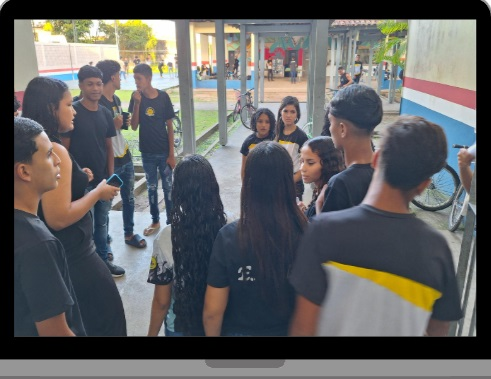
\includegraphics[width=2.26042in,height=\textheight,keepaspectratio]{fig6.jpg}
\end{center}

\begin{itemize}
\item
  \textbf{Direitos de Imagem}: Não é permitido gravar e expor pessoas
  sem sua expressa autorização, sobretudo em ambientes vulneráveis ou
  dentro do ambiente escolar, envolvendo menores de idade. A autorização
  documentada é um processo pedagógico sobre cidadania.
\item
  \textbf{Respeito à Dignidade}: O olhar crítico não é um olhar
  persecutório. A investigação de contradições sociais não deve expor
  trabalhadores locais, alunos ou professores a constrangimentos ou
  humilhações públicas.
\item
  \textbf{Crítica ao Sensacionalismo}: A linguagem das redes sociais
  frequentemente opera sob a lógica do espetáculo e da ``lacração''. A
  função do vídeo escolar é analítica. O professor deve combater
  exageros, mentiras descontextualizadas ou trilhas sonoras
  manipuladoras que reforcem preconceitos.
\item
  \textbf{Checagem de Informações}: Qualquer dado estatístico ou
  denúncia presente nos vídeos deve passar por rigorosa checagem de
  fatos, junto às equipes antes da edição final.
\end{itemize}

\bookmarksetup{startatroot}

\chapter{Considerações Finais}\label{considerauxe7uxf5es-finais}

A aplicação da Metodologia da Transitividade através da produção
audiovisual representa uma intervenção pedagógica vigorosa em prol de
uma escola efetivamente conectada à vida social. Ao longo deste guia
prático, evidenciou-se que o verdadeiro potencial do dispositivo móvel
na sala de aula não repousa no consumo passivo, mas na sua capacidade de
instrumentalizar o aluno na leitura crítica da realidade.

\begin{center}
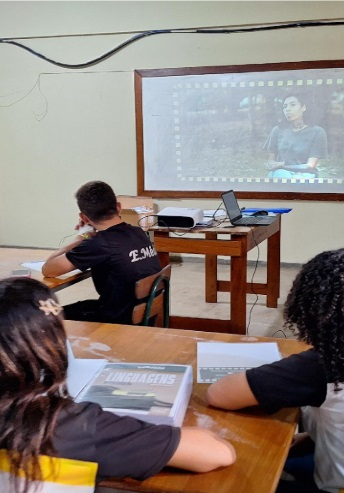
\includegraphics[width=2in,height=\textheight,keepaspectratio]{fig7.jpg}
\end{center}

Neste trajeto que vai da codificação visual do cotidiano aos diálogos
descodificadores, o estudante transita de uma postura observadora
ingênua, para uma postura investigativa, consciente e reflexiva.
Produzir um vídeo para redes sociais deixa de ser um mero ato de
exposição pessoal, para converter-se em um profundo exercício ético, de
autoria discursiva e intervenção cultural.

\subsection{Referência Base}\label{referuxeancia-base}

A organização estrutural, pedagógica e teórica deste e-book foi
consolidada a partir da sistematização de informações e análises
oriundas da Dissertação de Mestrado: O recurso do áudiovisual no ensino
de sociologia: o uso do celular na produção de minidocumentários para o
exercício da metodologia da transitividade.

\bookmarksetup{startatroot}

\chapter*{Referências
Bibliográficas}\label{referuxeancias-bibliogruxe1ficas}
\addcontentsline{toc}{chapter}{Referências Bibliográficas}

\markboth{Referências Bibliográficas}{Referências Bibliográficas}

Fonte: FREIRE, P. A Pedagogia do Oprimido, 2023.

FREIRE, P. Educação como Prática de Liberdade, 2025.

Machado Filho, Francisco. Como fazer Documentários, 2024.

ALVES, G. O cinema como experiência crítica, 2010.

\protect\phantomsection\label{refs}




\end{document}
